\subsubsection{Experimental Biophysics and Nanotechnology }
\index{Fritz, J\"urgen}

\paragraph{Research Team}
J\"urgen Fritz (Professor), Ioana Pera (Postdoc), Astrid Kronenberger (PhD student)\\

Our group is working in the field of experimental biophysics and nanotechnology. We are interested in the structure and interaction of single biomolecules and the detection of biomolecules with nanomechanical biosensors.
Both approaches aim for a better understanding of biomolecular systems on a fundamental level, for developing new bioanalytical tools, and exploring the application of biomolecules in nanotechnology. Current projects involve the visualization of single protein / DNA complexes and individual membrane channel proteins by atomic force microscopy, and developing sensors for directly measuring mechanical properties of cellular membranes. In addition, we work on applications of microfluidics for biosensing experiments and liposome separation\cite{Fritz2} and for trapping of DNA between microstructured electrodes for future molecular electronics and nanobiotechnology.


\paragraph{Highlights}


Our main method is the atomic force microscope (AFM) which enables one to image single molecules with high resolution on flat surfaces at ambient conditions but also in solution, which is especially interesting for biological samples. The AFM can resolve structures of nanometer dimension. In a collaboration with Prof. Muskhelishvili (IUB) we are looking at the details and molecular arrangements of single protein-DNA complexes. These ternary complexes consist of a specific double-stranded DNA, a RNA polymerase and an activator protein. All three are needed to initiate transcription, i.e. the transfer of a specific part of genetic information from DNA to RNA. A first paper on this project was published this year\cite{Fritz1}. The work on imaging membrane channel proteins (FhuA and OmpF) by AFM is ongoing. The two bottlenecks, the 2D crystallization of membrane proteins for AFM and the stable imaging of proteins in solution have still to be optimized.

A second focus of our research is on investigating mechanical properties of lipid bilayers by microfabricated cantilever sensors. Several interactions and processes in cellular biology change the mechanical properties of cellular membranes, e.g. vesicle budding, protein reconstitution, cholesterol insertion or virus docking. These processes lead to a change in membrane structure and composition and are associated with changes in membrane mechanical parameters such as curvature, area expansion or lateral pressure of lipid bilayers. Microfabricated cantilever sensors are known to sense the binding of biomolecules to their surface or the expansion of a molecular layer immobilized on their surface\cite{Fritz3}. By functionalizing the cantilevers of an array with artificial phospholipid bilayers, the interaction of molecules with these bilayers can be monitored by the bending of the cantilevers. Systems of interest are the chemical degradation of bilayers by enzymes (e.g. phospholipases) or insertion of pore forming molecules into the bilayer (e.g. melittin). Both interactions are of industrial or pharmacological relevance. First results will be published this year\cite{Fritz4}.




\begin{figure}[ht]
  \begin{center}
    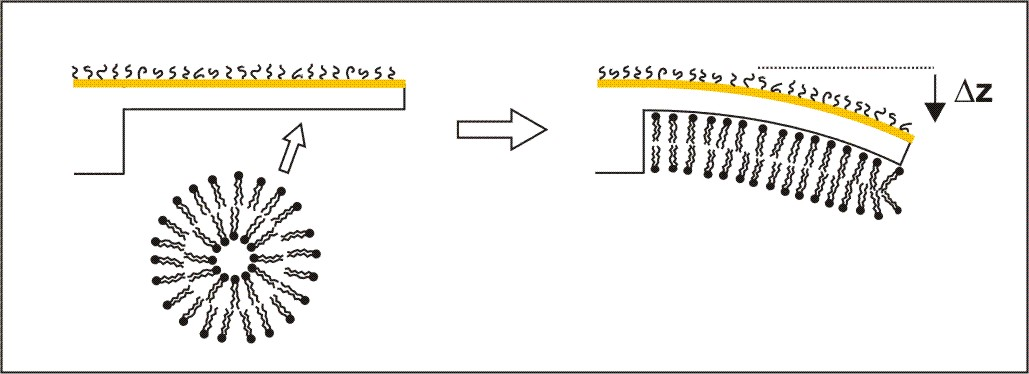
\includegraphics[width=\hsize]{Fritz/ProfFritz-Fig.jpg}
    \mycaption{Scheme of a microfabricated cantilever sensor detecting the formation of supported lipid bilayer by a mechanical bending of some nanometer.
)}\label{fig:Fritz}
   \end{center}
\end{figure}


\paragraph{Collaborations}
\begin{enumerate}
\item Prof. Winterhalter (IUB): microfluidics for electrophysiology and liposome separation
\item Prof. Wagner (IUB): microstructures for molecular electronics of biomolecules
\item Prof. Muskhelishvili (IUB): characterization of DNA/protein interactions by AFM
\end{enumerate}

\paragraph{Grants}
\begin{enumerate}
\item Funded by BMBF, \emph{Embedded Microsystems Bremen (EMB)}
\end{enumerate}
